\documentclass[tikz,border=8pt]{standalone}
\usepackage{amsmath}
\usetikzlibrary{arrows.meta,calc,decorations.markings}
\definecolor{ink}{HTML}{21352F}
\definecolor{teal}{HTML}{087F7B}
\definecolor{blue}{HTML}{4B77A8}
\definecolor{gold}{HTML}{C58B2A}
\definecolor{rose}{HTML}{B65A62}
\begin{document}
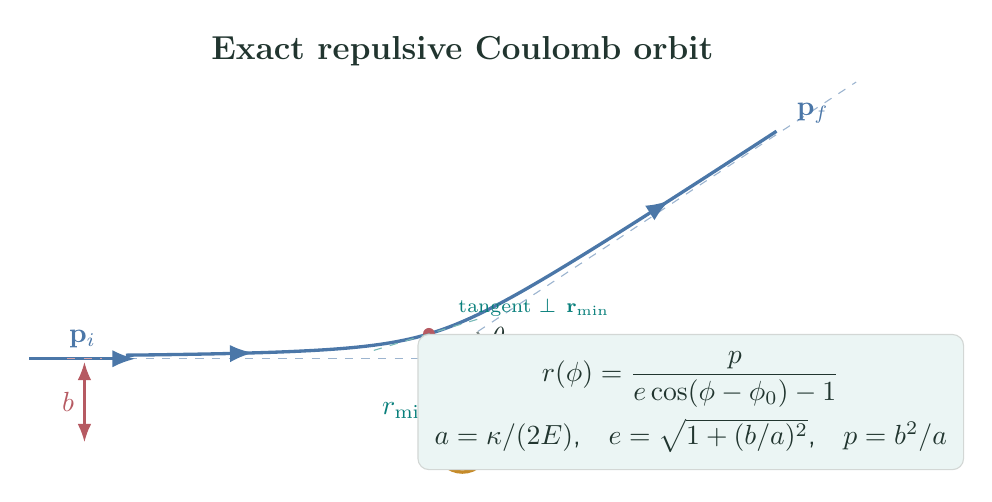
\begin{tikzpicture}[font=\sffamily,text=ink,>=Latex]
  % Exact plotted example: a=0.6, b=2 in common length units.
  \pgfmathsetmacro{\coulomba}{0.6}
  \pgfmathsetmacro{\impactb}{2.0}
  \pgfmathsetmacro{\ecc}{sqrt(1+(\impactb/\coulomba)^2)}
  \pgfmathsetmacro{\semilatus}{\impactb*\impactb/\coulomba}
  \pgfmathsetmacro{\scatterangle}{2*atan(\coulomba/\impactb)}
  \pgfmathsetmacro{\periangle}{(180+\scatterangle)/2}
  \pgfmathsetmacro{\closest}{\coulomba+sqrt(\coulomba^2+\impactb^2)}
  \pgfmathsetmacro{\plotscale}{0.55}
  \pgfmathsetmacro{\periX}{\plotscale*\closest*cos(\periangle)}
  \pgfmathsetmacro{\periY}{\plotscale*\closest*sin(\periangle)}
  \pgfmathsetmacro{\incomingY}{\plotscale*\impactb}
  \pgfmathsetmacro{\asymptoteX}{-\plotscale*\coulomba}

  \node[font=\bfseries\large] at (0,5.0)
    {Exact repulsive Coulomb orbit};
  \coordinate (N) at (0,0);
  \coordinate (A) at (\asymptoteX,\incomingY);
  \coordinate (P) at (\periX,\periY);

  % The two exact asymptotes generated by the same a and b.
  \draw[blue!55,dashed] (-5.5,\incomingY)--(A);
  \draw[blue!55,dashed] (A)--
    ({5.0},{5.0*tan(\scatterangle)
      +\plotscale*\impactb/cos(\scatterangle)});
  \draw[blue,very thick,->] (-5.5,\incomingY)--(-4.15,\incomingY)
    node[midway,above] {$\mathbf p_i$};

  % r(phi)=p/[e cos(phi-phi_0)-1], traversed from phi=165 deg
  % toward phi=45 deg. Both arrowheads follow the exact curve.
  \draw[blue,very thick,
        postaction={decorate},
        decoration={markings,
          mark=at position .18 with {\arrow{Latex}},
          mark=at position .82 with {\arrow{Latex}}}]
    plot[domain=165:45,samples=180,variable=\ph]
    ({\plotscale*
       (\semilatus/(\ecc*cos(\ph-\periangle)-1))*cos(\ph)},
     {\plotscale*
       (\semilatus/(\ecc*cos(\ph-\periangle)-1))*sin(\ph)});
  \node[blue] at (4.45,4.22) {$\mathbf p_f$};

  \fill[gold!24] (N) circle (.34);
  \draw[gold,very thick] (N) circle (.34);
  \node[font=\bfseries] at (N) {$+Ze$};

  \draw[<->,rose,thick] (-4.8,.04)--(-4.8,\incomingY-0.04)
    node[midway,left] {$b$};
  \draw[rose!55,dashed] (-5.02,\incomingY)--(-4.58,\incomingY);

  \draw[teal,thick,->] (N)--(P)
    node[midway,below left=1pt] {$r_{\min}$};
  \fill[rose] (P) circle (.075);
  \draw[teal!55,dashed] ($(P)+(-.7,-.21)$)--($(P)+(.7,.21)$);
  \node[font=\scriptsize,teal,anchor=south west] at ($(P)+(.25,.1)$)
    {tangent $\perp\,\mathbf r_{\min}$};

  \draw[ink!60,thick] ($(A)+(.62,0)$)
    arc[start angle=0,end angle=\scatterangle,radius=.62];
  \node at ($(A)+(.79,.28)$) {$\theta$};

  \node[draw=ink!20,fill=teal!8,rounded corners=4pt,
        inner sep=6pt,align=center] at (2.9,.55)
    {$\displaystyle
      r(\phi)=\frac{p}{e\cos(\phi-\phi_0)-1}$\\[3pt]
     $a=\kappa/(2E)$,\quad
     $e=\sqrt{1+(b/a)^2}$,\quad
     $p=b^2/a$};
\end{tikzpicture}
\end{document}
